\section{黎曼信赖域}
\label{sec:mfo-trust-region}

第~\ref{sec:mfo-newton}节的起点上，Newton步是上升方向；第~\ref{sec:mfo-pullback}节的$s=1$处，模型误差已经达到$\tfrac{5}{18}$。这两件事都说明，曲率模型只在有限的尺度内可信。第~\ref{chap:trust-region}章的信赖域正是处理这个问题的，本节回答它怎样搬到切空间上，又有哪些新的条件要核对。

\paragraph{主要思想}
在当前切空间的有限半径内近似最小化模型~\eqref{eq:mfo-model}：
\begin{equation}
 \min_{\bm{v}\in T_{\bm{x}}M}\ m_{\bm{x}}(\bm{v})\quad\text{s.t.}\quad\lVert\bm{v}\rVert_2\leq\Delta.
 \label{eq:mfo-rtr-subproblem}
\end{equation}
半径$\Delta$在切空间里度量，子问题是线性空间上的普通信赖域子问题。

得到候选步$\bm{v}$后，回缩到流形上，比较实际下降与预测下降：
\begin{equation}
 \rho=\frac{f(\bm{x})-f(R_{\bm{x}}(\bm{v}))}{m_{\bm{x}}(\bm{0})-m_{\bm{x}}(\bm{v})}.
 \label{eq:mfo-rtr-ratio}
\end{equation}
分子必须用回缩后的点，所以回缩造成的偏差也一并得到了检验。

接受和半径的规则沿用第~\ref{chap:trust-region}章：$\rho\geq\tfrac14$时接受，否则留在原地；$\rho<\tfrac14$时半径缩小为$\tfrac14$倍，$\rho\geq\tfrac34$且步到达边界时半径加倍（不超过上限$\Delta_{\max}$），其余情形半径不变。这样曲率模型只在获得检验的尺度内被使用。这就是\term{黎曼信赖域}（Riemannian trust region）方法。

图~\ref{fig:mfo-rtr-disc}画出贯穿例第$0$轮的几何。紫色椭圆是切平面上半径为$1$的圆盘，它的回缩像是球面上的绿色小圆。候选步在切平面上产生，回缩后落在绿圈之内或之上。

\begin{BookInlineFigure}
 \centering
 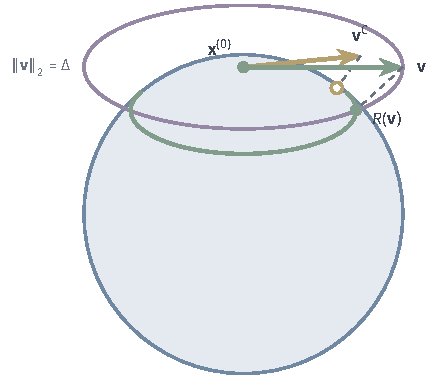
\includegraphics[width=74.0mm]{figures/05-optimization/06-constrained-optimization/tikz/mfo-rtr-disc/figure.pdf}
 \caption{切平面上的信赖域及其回缩像。紫色是切平面上半径$\Delta=1$的圆的边界，绿色闭曲线是它在归一化回缩下的像。黄箭头是Cauchy步$\bm{v}^{\mathrm{C}}$，绿箭头是截断CG得到的步$\bm{v}$，虚线是回缩，实心点是接受的新点。}
 \label{fig:mfo-rtr-disc}
\end{BookInlineFigure}

\subsection{子问题的求解}
\label{sec:mfo-rtr-subproblem}

\paragraph{Cauchy步}
最便宜的办法是沿负梯度在半径内最小化模型，这就是第~\ref{chap:trust-region}章的\term{Cauchy步}（Cauchy step）。记沿负梯度的曲率为
\[
 \kappa=\frac{\langle\bm{g},\bm{H}\bm{g}\rangle}{\lVert\bm{g}\rVert_2^2},
\]
当$\kappa>0$且$\lVert\bm{g}\rVert_2/\kappa<\Delta$时取$\bm{v}^{\mathrm{C}}=-\bm{g}/\kappa$，否则走到边界。

第~\ref{chap:trust-region}章证明了它的预测下降满足下面的下限，切空间上的证明一字不改：
\begin{equation}
 m(\bm{0})-m(\bm{v}^{\mathrm{C}})\geq\frac12\lVert\bm{g}\rVert_2\min\Bigl\{\Delta,\ \frac{\lVert\bm{g}\rVert_2}{\lVert\bm{H}\rVert_2}\Bigr\}.
 \label{eq:mfo-cauchy-decrease}
\end{equation}

\paragraph{截断共轭梯度}
只用Cauchy步相当于梯度法，为了利用曲率，用第~\ref{chap:trust-region}章的\term{截断共轭梯度法}（truncated conjugate gradient）在切空间内迭代。迭代从$\bm{v}=\bm{0}$开始，第一步就是Cauchy步的方向，之后模型值单调下降，所以最终的预测下降不低于Cauchy步。

三种情形下停止：残差足够小；遇到负曲率时沿当前方向走到边界；下一步要越界时截断在边界。残差容差取
\begin{equation}
 \lVert\bm{r}\rVert_2\leq\lVert\bm{r}_0\rVert_2\min\bigl\{\lVert\bm{r}_0\rVert_2^{\theta},\ \varkappa\bigr\},
 \label{eq:mfo-rtr-forcing}
\end{equation}
其中$\theta>0$，$\varkappa\in(0,1)$。

\needspace{6\baselineskip}
\paragraph{变量}
\begin{itemize}
 \item $\bm{x}^{(t)}$：当前点；$\Delta^{(t)}$：半径；$\bm{g},\bm{H}$：当前切空间基下的梯度坐标和Hessian。
 \item $\bm{v}_j$：内层的当前步，$\bm{r}_j$：残差$\bm{H}\bm{v}_j+\bm{g}$，$\bm{p}_j$：共轭方向，均为二维坐标。
 \item 参数：$\theta=1$，$\varkappa=0.1$。
\end{itemize}

\paragraph{初始化}
例中$\bm{x}^{(0)}=\tfrac13(2,2,1)^\top$，$\Delta^{(0)}=1$。由第~\ref{sec:mfo-newton}节的数据，
\[
 \bm{g}=\begin{bmatrix}2/9\\-8/9\end{bmatrix},\qquad
 \bm{H}=\begin{bmatrix}1&-10/9\\-10/9&2/3\end{bmatrix}.
\]
内层初始化为$\bm{v}_0=\bm{0}$，$\bm{r}_0=\bm{g}$，$\bm{p}_0=-\bm{g}$。

\needspace{6\baselineskip}
\paragraph{每轮更新}
\begin{enumerate}
 \item 计算$\kappa_j=\langle\bm{p}_j,\bm{H}\bm{p}_j\rangle$。例中第$0$步$\bm{H}\bm{p}_0\approx(-1.2099,0.8395)^\top$，$\kappa_0\approx1.0151>0$。

 \item 若$\kappa_j\leq0$，沿$\bm{p}_j$走到边界后结束内层。否则取$\alpha_j=\lVert\bm{r}_j\rVert_2^2/\kappa_j$，并算$\bm{v}_{j+1}=\bm{v}_j+\alpha_j\bm{p}_j$。例中$\alpha_0=\tfrac{153}{185}\approx0.8270$，
 \[
  \bm{v}_1=\Bigl(-\frac{34}{185},\ \frac{136}{185}\Bigr)^\top\approx(-0.1838,\ 0.7351)^\top.
 \]
 它的长度约为$0.7578<1$，不越界，这就是Cauchy步，预测下降$0.3471$。

 \item 更新残差和方向：
 \[
  \begin{gathered}
  \bm{r}_{j+1}=\bm{r}_j+\alpha_j\bm{H}\bm{p}_j,\qquad
  \beta_j=\frac{\lVert\bm{r}_{j+1}\rVert_2^2}{\lVert\bm{r}_j\rVert_2^2},\\
  \bm{p}_{j+1}=-\bm{r}_{j+1}+\beta_j\bm{p}_j.
  \end{gathered}
 \]
 例中
 \[
  \bm{r}_1\approx(-0.7784,\ -0.1946)^\top,\quad\beta_0\approx0.7668,\quad\bm{p}_1\approx(0.6080,\ 0.8762)^\top.
 \]

 \item 例中第$1$步$\kappa_1\approx-0.302<0$，遇到负曲率。解$\lVert\bm{v}_1+\tau\bm{p}_1\rVert_2=1$，得$\tau\approx0.3023$，于是
 \[
  \bm{v}=\bm{v}_1+\tau\bm{p}_1=(0,\ 1)^\top.
 \]
 所以$\bm{v}=\bm{E}_2$，正好是切空间的基向量，内层结束。

 \item 算预测下降。例中$m(\bm{v})-f(\bm{x})=-\tfrac89+\tfrac13$，所以预测下降$\tfrac59$。

 \item 回缩并算$\rho$。例中$\bm{x}^{(0)}+\bm{E}_2=\tfrac13(4,1,-1)^\top$，长度$\sqrt2$，
 \[
  R_{\bm{x}^{(0)}}(\bm{v})=\frac{(4,1,-1)^\top}{3\sqrt2}\approx(0.9428,0.2357,-0.2357)^\top,\qquad f=\frac{11}{18}.
 \]
 实际下降$\tfrac89-\tfrac{11}{18}=\tfrac{5}{18}$，由式~\eqref{eq:mfo-rtr-ratio}得$\rho=\tfrac12$。

 \item 按规则更新。例中$\rho=\tfrac12\in[\tfrac14,\tfrac34)$，接受这一步，半径保持$1$。
\end{enumerate}

对比只用Cauchy步：其回缩点的目标值是$0.6684$，$\rho\approx0.635$，实际下降$0.2205$；截断CG多用一次Hessian--向量乘积，实际下降增加到$0.2778$。负曲率方向在这里提供了额外的下降，而第~\ref{sec:mfo-newton}节的Newton方向恰恰是上升的。

图~\ref{fig:mfo-rtr-model}把这一轮放回切平面坐标。在原点附近模型与拉回的等值线几乎重合，到半径$1$的边界上两者已明显不同。

\begin{BookInlineFigure}
 \centering
 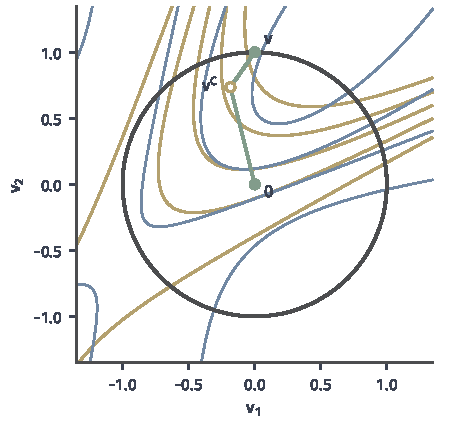
\includegraphics[width=78.0mm]{figures/05-optimization/06-constrained-optimization/matplotlib/mfo-rtr-model/figure.pdf}
 \caption{$\bm{x}^{(0)}$处切平面坐标下的模型（黄）与拉回目标（蓝）的等值线，两组曲线使用相同的水平。深灰圆是半径$\Delta=1$的边界，绿色折线是截断CG的路径，空心点是Cauchy步。模型不定，等值线不闭合。}
 \label{fig:mfo-rtr-model}
\end{BookInlineFigure}

后面几轮的结果如表~\ref{tab:mfo-rtr-run}。第$1$轮起都在内部收敛，$\rho$迅速接近一，模型变得可信，与Newton法的快速局部收敛衔接。第$4$轮$\lVert\bm{g}\rVert_2$约为$9.4\times10^{-11}$，低于容差，迭代结束，最终得到$\bm{x}^{(4)}\approx\bm{e}_1$。

\begin{BookInlineTable}
 \centering
 \caption{贯穿例的黎曼信赖域，$\Delta^{(0)}=1$。}
 \label{tab:mfo-rtr-run}
 \begin{tabular}{llllll}
  \toprule
  $t$ & $f(\bm{x}^{(t)})$ & $\lVert\bm{g}^{(t)}\rVert_2$ & 内层结束方式 & 预测下降 & $\rho$\\
  \midrule
  $0$ & $0.8889$ & $0.9162$ & 负曲率 & $0.5556$ & $0.500$\\
  $1$ & $0.6111$ & $0.7115$ & 残差 & $0.1279$ & $0.844$\\
  $2$ & $0.5031$ & $0.0928$ & 残差 & $3.15\times10^{-3}$ & $0.994$\\
  $3$ & $0.5000$ & $4.68\times10^{-4}$ & 残差 & $1.04\times10^{-7}$ & $1.000$\\
  \bottomrule
 \end{tabular}
\end{BookInlineTable}

\paragraph{进展条件}
实际运行中要求候选步的模型下降至少达到Cauchy步的某个比例，这是全局收敛分析的常用条件：存在$c\in(0,\tfrac12]$，使得
\begin{equation}
 m(\bm{0})-m(\bm{v})\geq c\lVert\bm{g}\rVert_2\min\Bigl\{\Delta,\ \frac{\lVert\bm{g}\rVert_2}{\beta}\Bigr\},
 \label{eq:mfo-cauchy-fraction}
\end{equation}
这里$\beta\geq\lVert\bm{H}\rVert_2$。截断CG自动满足它，取$c=\tfrac12$。

这个条件只针对一阶进展。更强的二阶驻点保证要求子问题求解器能处理负曲率。截断CG从$\bm{v}=\bm{0}$出发，第一步方向是$-\bm{g}$，当$\bm{g}=\bm{0}$时立即停止。贯穿例中恰好落在鞍点$\bm{e}_2$时，$\bm{g}=\bm{0}$，切向曲率有$-1$，但截断CG返回零步，迭代就此停住。

要逃出这样的点，须在小梯度时计算$\bm{H}$的最小特征值及其特征向量，并沿该方向走一步，这个步称为特征步。第~\ref{chap:saddle-points}章的讨论在切空间上同样适用。

\subsection{模型与回缩条件}
\label{sec:mfo-rtr-conditions}

\paragraph{近似误差进入比值}
由式~\eqref{eq:mfo-rtr-ratio}，因为$m(\bm{0})=f(\bm{x})$，比值的偏差可以写成
\begin{equation}
 1-\rho=\frac{\hat{f}_{\bm{x}}(\bm{v})-m_{\bm{x}}(\bm{v})}{m_{\bm{x}}(\bm{0})-m_{\bm{x}}(\bm{v})}.
 \label{eq:mfo-rho-gap}
\end{equation}
分子是拉回目标与模型的差，分母是预测下降，所有误差都集中在分子。分子由三部分组成：回缩对一阶和二阶信息的近似、$\bm{H}$与真实曲率的差、拉回函数的高阶余项。

分母受子问题求解精度的影响。子问题解得差，分母偏小，比值波动就大。所以这个比值同时检验了模型、回缩和子问题三者。

\paragraph{达到小梯度}
下面的定理说明，什么样的近似误差足以保证梯度变小。这里假定拉回目标与模型之差被二次函数界住。

\begin{theorem}[黎曼信赖域的迭代界]
 \label{thm:mfo-rtr-complexity}
 设$f$有下界$f^\star$，所有迭代满足式~\eqref{eq:mfo-cauchy-fraction}，$\lVert\bm{H}^{(t)}\rVert_2\leq\beta$，并且存在$C\geq\beta$，使
 \begin{equation}
  \bigl\lvert\hat{f}_{\bm{x}^{(t)}}(\bm{v})-m_{\bm{x}^{(t)}}(\bm{v})\bigr\rvert\leq\frac C2\lVert\bm{v}\rVert_2^2,\qquad\lVert\bm{v}\rVert_2\leq\Delta_{\max}.
  \label{eq:mfo-model-error}
 \end{equation}
 按本节规则更新半径。若前$T$轮都有$\lVert\bm{g}^{(t)}\rVert_2\geq\varepsilon$，令
 \begin{equation}
  \underline{\Delta}=\min\Bigl\{\Delta^{(0)},\ \frac{c\varepsilon}{8C}\Bigr\},
  \label{eq:mfo-rtr-radius-floor}
 \end{equation}
 则
 \begin{equation}
  T\leq\frac{6\bigl(f(\bm{x}^{(0)})-f^\star\bigr)}{c\,\varepsilon\,\underline{\Delta}}+\frac12\log_2\frac{\Delta^{(0)}}{\underline{\Delta}}.
  \label{eq:mfo-rtr-complexity}
 \end{equation}
 所以小的$\varepsilon$对应的迭代次数为$O(1/\varepsilon^2)$。
\end{theorem}

\begin{proof}
 第一步证明半径小时比值接近一。设$\lVert\bm{g}\rVert_2\geq\varepsilon$，并设$\Delta\leq c\varepsilon/(2C)$。因为$c\leq\tfrac12$，$C\geq\beta$，所以$\Delta$不超过$\lVert\bm{g}\rVert_2/\beta$，式~\eqref{eq:mfo-cauchy-fraction}给出预测下降至少为$c\varepsilon\Delta$。

 再由式~\eqref{eq:mfo-rho-gap}和式~\eqref{eq:mfo-model-error}，并用$\lVert\bm{v}\rVert_2\leq\Delta$，得到
 \[
  \lvert1-\rho\rvert\leq\frac{C\Delta^2/2}{c\varepsilon\Delta}=\frac{C\Delta}{2c\varepsilon}\leq\frac14.
 \]
 于是$\rho\geq\tfrac34$，半径不会缩小。

 第二步给出半径的下界。半径只在$\rho<\tfrac14$时缩小，此时一定有$\Delta>c\varepsilon/(2C)$，缩小后仍大于$c\varepsilon/(8C)$。因此所有轮都有$\Delta^{(t)}\geq\underline{\Delta}$。

 第三步数接受的轮数$T_{\mathrm{a}}$。接受时$\rho\geq\tfrac14$，再用预测下降的下限，并用$\underline{\Delta}\leq\varepsilon/\beta$，得到
 \[
  f(\bm{x}^{(t)})-f(\bm{x}^{(t+1)})\geq\frac14c\varepsilon\underline{\Delta}.
 \]
 目标总下降量不超过$f(\bm{x}^{(0)})-f^\star$，所以
 \[
  T_{\mathrm{a}}\leq\frac{4\bigl(f(\bm{x}^{(0)})-f^\star\bigr)}{c\varepsilon\underline{\Delta}}.
 \]

 第四步数拒绝的轮数$T_{\mathrm{r}}$。每次拒绝半径乘$\tfrac14$，每次接受半径至多乘$2$，所以
 \[
  \underline{\Delta}\leq\Delta^{(T)}\leq\Delta^{(0)}\,2^{T_{\mathrm{a}}}\,4^{-T_{\mathrm{r}}}.
 \]
 取对数得
 \[
  T_{\mathrm{r}}\leq\frac12T_{\mathrm{a}}+\frac12\log_2\frac{\Delta^{(0)}}{\underline{\Delta}}.
 \]

 把$T=T_{\mathrm{a}}+T_{\mathrm{r}}$合起来，就得到式~\eqref{eq:mfo-rtr-complexity}。
\end{proof}

定理的假设分三项，各起一种作用。式~\eqref{eq:mfo-cauchy-fraction}保证分母足够大；$\lVert\bm{H}\rVert_2\leq\beta$保证小半径时走到边界的量级被正确估计；式~\eqref{eq:mfo-model-error}保证分子足够小。

这个假设对回缩的要求不高。把式~\eqref{eq:mfo-pullback-smooth}类型的双侧上界与$\lVert\bm{H}\rVert_2\leq\beta$相加，就得到式~\eqref{eq:mfo-model-error}，这时$\bm{H}$甚至不必是真实的Hessian，例如用$\bm{H}=\bm{0}$也行，此时算法退化为带半径控制的梯度法。在紧流形上，光滑目标和光滑回缩自动满足该假设。

\paragraph{二阶驻点与快速局部收敛}
定理只说梯度变小。要达到近似二阶驻点，即$\bm{H}\succeq-\varepsilon_H\bm{I}$，需要额外条件：$\bm{H}$在拉回Hessian的一定精度内，模型误差有三次界，子问题在负曲率时能产生下降正比于负曲率立方的步。在这些条件下，迭代次数的量级为$O(\max\{\varepsilon^{-2}\varepsilon_H^{-1},\varepsilon_H^{-3}\})$，证明沿用定理~\ref{thm:mfo-rtr-complexity}的结构并加入负曲率情形，读者可查阅\scite{math-boumal2023optimization}。

即使达到了二阶驻点，也不能断言是局部极小。第~\ref{sec:mfo-optimality}节的$x_2^3$例子满足二阶必要条件却不是局部极小。近似二阶驻点只是必要条件的数值形式。

快速局部收敛需要模型足够精确。若迭代收敛到非退化的极小点，$\bm{H}^{(t)}$是真实的黎曼Hessian，并用式~\eqref{eq:mfo-rtr-forcing}控制内层精度，那么$\rho\to1$，半径不再起作用，方法变成非精确Newton，局部收敛阶至少是$\min\{1+\theta,2\}$。证明需要回缩与Hessian的局部误差估计，这里只说明机制：第~\ref{sec:mfo-pullback}节的附加项正比于$\lVert\bm{g}\rVert_2$，一般回缩也不破坏这一速度。

图~\ref{fig:mfo-rtr-history}是$n=300$的问题。半径初值$2$过大，第$0$轮$\rho\approx0.20$被拒绝，半径缩小到$0.5$；第$1$轮$\rho\approx0.80$，半径扩大到$1$，此后半径保持不变。最后几轮$\rho\approx1$，梯度范数快速下降。

\begin{BookInlineFigure}
 \centering
 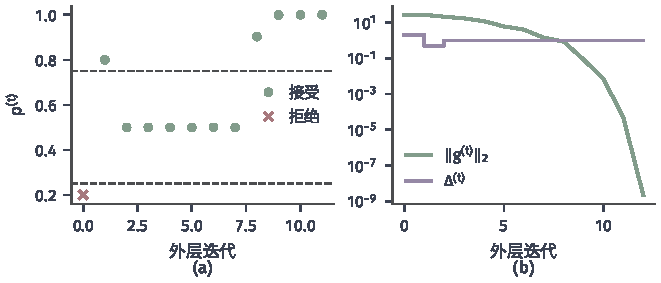
\includegraphics[width=112.0mm]{figures/05-optimization/06-constrained-optimization/matplotlib/mfo-rtr-history/figure.pdf}
 \caption{$n=300$，$\bm{A}$的特征值在$1$到$100$之间等距，随机起点固定，$\theta=1$，$\varkappa=0.1$，$\Delta^{(0)}=2$。(a)~各轮的比值$\rho$，绿点接受，红叉拒绝，两条虚线是$\tfrac14$与$\tfrac34$。(b)~梯度范数（绿）和半径（紫）。}
 \label{fig:mfo-rtr-history}
\end{BookInlineFigure}
